\documentclass[11pt,a4paper]{article}

% ============================================================================
% Standard arXiv-Compatible Packages (TeX Live 2023/2024/2025 safe)
% ============================================================================
\usepackage[utf8]{inputenc}
\usepackage[T1]{fontenc}
\usepackage[margin=1in]{geometry}
\usepackage{amsmath,amssymb,amsfonts,amsthm}
\usepackage{booktabs}
\usepackage{multirow}
\usepackage{tabularx}
\usepackage{graphicx}
\usepackage{xcolor}
\usepackage{tikz}
\usepackage{pgfplots}
\pgfplotsset{compat=1.18}
\usetikzlibrary{arrows.meta,positioning,shapes.geometric,fit,calc,backgrounds}
\usepackage{enumitem}
\usepackage{listings}
\usepackage{microtype}
\usepackage[colorlinks=true,linkcolor=blue!60!black,citecolor=blue!60!black,urlcolor=blue!60!black]{hyperref}

% Theorem / Invariant Environments
\newtheorem{invariant}{Architectural Invariant}
\newtheorem{proposition}{Proposition}
\newtheorem{definition}{Definition}

% Code Listing Style
\definecolor{codebg}{RGB}{248,249,250}
\definecolor{codeframe}{RGB}{220,224,230}
\definecolor{codekw}{RGB}{0,92,197}
\definecolor{codecmt}{RGB}{106,115,125}
\definecolor{codestr}{RGB}{3,47,98}

\lstdefinestyle{heurionspec}{
  backgroundcolor=\color{codebg},
  frame=single,
  rulecolor=\color{codeframe},
  basicstyle=\ttfamily\footnotesize,
  keywordstyle=\color{codekw}\bfseries,
  commentstyle=\color{codecmt}\itshape,
  stringstyle=\color{codestr},
  breaklines=true,
  columns=fullflexible,
  keepspaces=true,
  showstringspaces=false,
  aboveskip=6pt,
  belowskip=6pt
}

% Title and Author Metadata
\title{\textbf{Heurion 2.0: A Contract-Guarded Dual-Surface Architecture with Self-Evolving Memory for Citation-Grounded Clinical Research Authoring}}

\author{
  Hui Zhao\textsuperscript{1,*} \qquad Dong Qian\textsuperscript{2,*} \\[4pt]
  \small \textsuperscript{1}Heurion \\
  \small \textsuperscript{2}Department of Radiation Oncology, The First Affiliated Hospital of USTC, \\
  \small Division of Life Sciences and Medicine, University of Science and Technology of China, Hefei, China \\
  \small \textsuperscript{*}Corresponding authors: Dong Qian (\texttt{qiandong@ustc.edu.cn}), Hui Zhao (\texttt{huizhao@heurion.org})
}

\date{October 2026}

\begin{document}
\maketitle

% ============================================================================
% ABSTRACT
% ============================================================================
\begin{abstract}
Autonomous large language model (LLM) agents have achieved remarkable success in software engineering via free-form shell execution and direct file manipulation. However, transplanting this ``script-and-audit'' paradigm to high-stakes scientific and clinical research introduces severe failure modes: destructive formatting drift in Office Open XML (\texttt{.docx}/\texttt{.pptx}) manuscripts, silent overwriting of concurrent human edits, fabricated bibliographic identifiers (DOIs/PMIDs) or ungrounded statistical assertions, exposure of Protected Health Information (PHI), and repetitive guard failures across authoring sessions.

We present \textbf{Heurion 2.0}, a collaborative clinical research and scientific authoring platform built upon a \emph{Contract-Guarded Dual-Surface Architecture} and a \emph{Three-Layer Self-Evolving Memory System}. First, rather than allowing agents to mutate raw document files via ad-hoc scripts, Heurion 2.0 maintains a single Conflict-free Replicated Data Type (CRDT) source of truth (ProseMirror + Yjs) with lifecycle-stable block addressing (\texttt{\{\#id\}}). It exposes a synchronized dual surface: a rich-text/slide editor for human researchers and a compact Annotated Markdown projection with guarded structural primitives for AI agents, supporting per-turn selective undo in CRDT space and byte-preserving OOXML patch export for unmodified regions. Second, to ground manuscript evidence in verified sources, pre-write syntactic guards block unregistered inline citations while a multi-agent verification pipeline (\texttt{literature\_researcher}, \texttt{biostatistician}, \texttt{fact\_checker}) aligns manuscript sentences against PubMed abstracts and PubMed Central (PMC) full texts. Third, a privacy-preserving clinical research pipeline enforces dual-stage PHI redaction, pseudonymous subject mapping (\texttt{P001}), read-only Personal Health Record (PHR) red-lines, and CI-enforced Human-AI Permission Symmetry ($\mathcal{E}_{\text{REST}} = \phi(\mathcal{E}_{\text{MCP}}) \sqcup \mathcal{E}_{\text{NOT\_FOR\_AI}}$). Finally, a three-layer self-evolution mechanism combines side-effect-free pre-flight probes (\texttt{doc\_validate}), dual-track declarative/procedural memory crystallized from runtime execution signals, and background meta-strategy distillation. On 50 trials over a synthetic protocol template, the export reproduced the checked untouched blocks verbatim, and the pre-write guards intercepted every stale block overwrite and every unregistered citation in our test set at sub-millisecond latency ($0.168\,\text{ms}$ validation, $0.351\,\text{ms}$ edit), and rapid convergence of guard rejections to zero within three authoring sessions.
\end{abstract}

\vspace{4pt}
\noindent\textbf{Keywords:} Collaborative AI Agents, CRDT Co-Editing, Clinical Research Informatics, Citation Verification, Self-Evolving Memory, Human-AI Permission Symmetry

% ============================================================================
% 1. INTRODUCTION
% ============================================================================
\section{Introduction}
\label{sec:intro}

Clinical and biomedical research workflows demand an extraordinary degree of rigor, traceability, and regulatory compliance. A single clinical study typically spans patient longitudinal record curation, cohort screening, biostatistical modeling (e.g., baseline Table~1 generation, Kaplan--Meier survival curves, Cox proportional hazards regression, CONSORT flow diagrams), and the iterative authoring of peer-reviewed manuscripts (\texttt{.docx}) and academic presentation decks (\texttt{.pptx}) \cite{schulz2010consort,vandenbroucke2007strobe}. While recent agentic systems have demonstrated strong capabilities in code generation \cite{yang2024sweagent,wang2024openhands} and open-domain literature synthesis \cite{shao2024storm,skarlinski2024paperqa2}, deploying autonomous agents into real-world clinical research environments exposes four fundamental architectural barriers:

\begin{enumerate}[leftmargin=1.5em,itemsep=2pt]
  \item \textbf{The Free-Form File Mutation Trap:} First-generation document agents treat \texttt{.docx} and \texttt{.pptx} files as opaque disk artifacts manipulated via generated Python scripts (e.g., \texttt{python-docx}) followed by post-hoc quality audits. In practice, script-based rewrites strip publisher XML attributes, lose paragraph addressing identifiers (\texttt{w14:paraId}) during LibreOffice layout passes, suffer from punctuation/whitespace reproduction drift in full-block replacements, and cannot selectively undo an AI turn once a human co-author makes concurrent edits.
  \item \textbf{Citation Fabrication and Ungrounded Clinical Claims:} LLMs frequently hallucinate plausible-looking Digital Object Identifiers (DOIs), PubMed IDs (PMIDs), or numerical hazard ratios ($HR$) and $p$-values \cite{ji2023survey,walters2023fabrication}. Post-hoc prompting alone cannot guarantee that every inline reference corresponds to a verified bibliographic record or that statistical assertions match the cited source text.
  \item \textbf{Patient Privacy (PHI) Exposure and Permission Asymmetry:} Clinical investigators work with raw electronic medical records containing Protected Health Information (patient names, national ID numbers, admission codes, phone numbers). Passing unredacted records to external LLMs conflicts with health-data protection law in both jurisdictions we target: China's Personal Information Protection Law (PIPL) classifies medical and health information as sensitive personal information that may be processed only for a specific purpose, with separate consent and strict protective measures, and imposes additional conditions on cross-border transfer \cite{pipl2021}; the U.S. HIPAA Privacy Rule restricts disclosure of PHI unless it is de-identified, for example by removing the 18 Safe Harbor identifiers \cite{hipaa1996}. Conversely, granting agents unrestricted database or shell access creates severe privilege-escalation risks.
  \item \textbf{Cross-Session Amnesia and Memory Pollution:} When an agent encounters a structural guard rejection (e.g., attempting to overwrite a human-edited block or inserting an unregistered citation) or when a clinician reverts an AI turn, stateless agents repeat the exact same operational failure in subsequent turns. Naively appending all historical observations into a single flat memory pool mixes subjective user writing preferences with hard operational constraints, exhausting context budgets with low-utility noise \cite{shinn2023reflexion,packer2023memgpt}.
\end{enumerate}

\subsection{Lessons from First-Generation Post-Hoc Auditing (Heurion v1)}
Prior to developing Heurion 2.0, we deployed a first-generation architecture (\emph{Heurion v1 / S-Series}) in which an agent operated inside a workspace shell, invoking Python utilities to unpack, mutate, and repackage \texttt{.docx} archives while a post-turn supervisor audited text survival rates, paragraph drift, and DOI validity. Empirical deployment revealed that \emph{post-hoc auditing is fundamentally too late}: by the time an audit script detects a broken XML run or an unverified citation, the corrupted state has already been written, requiring expensive rollbacks or brittle three-way merges against concurrent browser edits.

\subsection{The Heurion 2.0 Paradigm Shift and Contributions}
Heurion 2.0 resolves these limitations by shifting from \emph{post-hoc file auditing} to \emph{pre-write structural contracts over a shared CRDT core}, coupled with a \emph{signal-driven self-evolving execution harness}. Our primary contributions are fourfold:

\begin{itemize}[leftmargin=1.5em,itemsep=2pt]
  \item \textbf{Contract-Guarded Dual-Surface CRDT Engine (Section~\ref{sec:dualsurface}):} We design a unified ProseMirror + Yjs document core with persistent block addressing (\texttt{\{\#id\}}), node-level optimistic concurrency control (\texttt{base\_rev}), minimal-diff XML fragment updates that preserve inline marks and comment anchors, per-turn selective CRDT undo (\texttt{revertTurn}), and 100\% byte-preserving OOXML patch export for untouched document regions.
  \item \textbf{Pre-Write Citation and PHI Guards (Section~\ref{sec:evidence}):} We enforce a syntactic pre-write ban on raw inline DOIs/PMIDs, requiring registration via Crossref, PubMed, and OpenAlex into atomic citation nodes (\texttt{[@c:id]}), and a deterministic checksum-backed PHI scanner that redacts patient identifiers before clinical text enters LLM context. We additionally describe, as system components without quantitative evaluation in this paper, a multi-agent sentence-level claim verification pipeline against PubMed abstracts and PMC full texts and a sandboxed biostatistical toolchain.
  \item \textbf{Three-Layer Self-Evolving Agent Architecture (Section~\ref{sec:evolution}):} We introduce a hierarchical adaptation loop comprising (Layer~1) side-effect-free pre-flight validation probes (\texttt{doc\_validate} / \texttt{dry\_run}), (Layer~2) a dual-track memory architecture that physically separates human-approved declarative preferences from runtime-crystallized procedural strategies ranked by token-normalized utility, and (Layer~3) background meta-strategy distillation into dynamic agent profile overlays.
  \item \textbf{CI-Enforced Human-AI Permission Symmetry (Section~\ref{sec:parity}):} We establish, and mechanically check via an automated parity test over the router table, an architectural invariant across all platform endpoints: every REST capability either maps 1-to-1 to an in-process Model Context Protocol (MCP) tool executing under the user's exact RBAC identity, or is explicitly justified in a restricted exclusion set, with high-risk mutations gated by human-only confirmation cards.
\end{itemize}

% ============================================================================
% 2. SYSTEM OVERVIEW & ARCHITECTURAL INVARIANTS
% ============================================================================
\section{System Overview and Design Principles}
\label{sec:overview}

Figure~\ref{fig:architecture} illustrates the end-to-end architecture of Heurion 2.0. The platform strictly decouples \emph{structured document/slide state mutation} from \emph{sandboxed statistical computation}.

\begin{figure}[t]
\centering
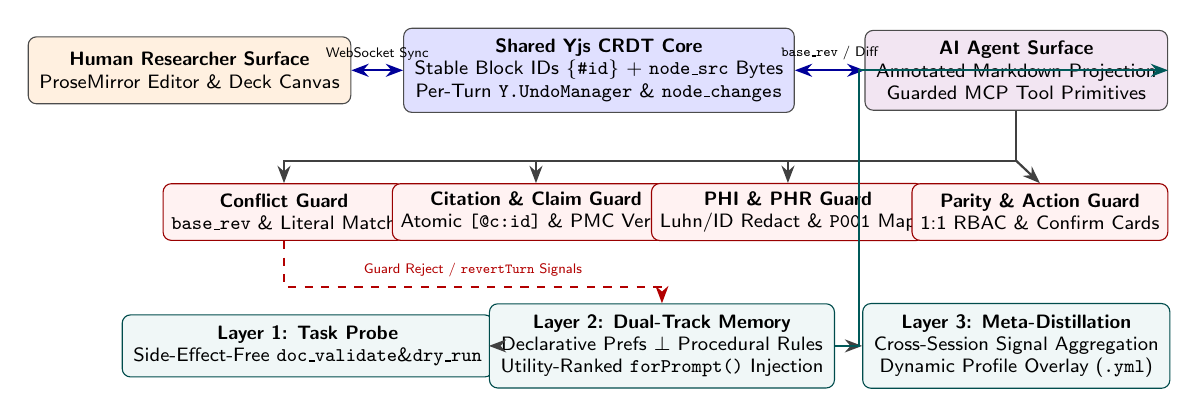
\begin{tikzpicture}[
  font=\sffamily\scriptsize,
  box/.style={draw=black!70, rounded corners=3pt, fill=white, align=center, minimum height=0.85cm, inner sep=4pt},
  pillar/.style={draw=blue!50!black, fill=blue!4, rounded corners=4pt, inner sep=6pt},
  guard/.style={draw=red!60!black, fill=red!5, rounded corners=3pt, align=center, minimum height=0.72cm, inner sep=3pt},
  evol/.style={draw=teal!60!black, fill=teal!6, rounded corners=3pt, align=center, minimum height=0.75cm, inner sep=4pt},
  arr/.style={-{Stealth[length=2.2mm]}, thick, draw=black!75},
  darr/.style={{Stealth[length=2.2mm]}-{Stealth[length=2.2mm]}, thick, draw=blue!60!black}
]

% Top Layer: Dual Surface
\node[box, fill=orange!12, minimum width=3.6cm] (human) at (0, 3.6) {\textbf{Human Researcher Surface}\\ProseMirror Editor \& Deck Canvas};
\node[box, fill=blue!12, minimum width=4.2cm] (crdt) at (5.2, 3.6) {\textbf{Shared Yjs CRDT Core}\\Stable Block IDs \texttt{\{\#id\}} + \texttt{node\_src} Bytes\\Per-Turn \texttt{Y.UndoManager} \& \texttt{node\_changes}};
\node[box, fill=violet!10, minimum width=3.8cm] (agentview) at (10.5, 3.6) {\textbf{AI Agent Surface}\\Annotated Markdown Projection\\Guarded MCP Tool Primitives};

\draw[darr] (human) -- node[above, font=\sffamily\tiny]{WebSocket Sync} (crdt);
\draw[darr] (crdt) -- node[above, font=\sffamily\tiny]{\texttt{base\_rev} / Diff} (agentview);

% Middle Layer: Pre-Write Structural Guards
\node[guard, minimum width=2.9cm] (g1) at (1.2, 1.8) {\textbf{Conflict Guard}\\\texttt{base\_rev} \& Literal Match};
\node[guard, minimum width=2.9cm] (g2) at (4.4, 1.8) {\textbf{Citation \& Claim Guard}\\Atomic \texttt{[@c:id]} \& PMC Verify};
\node[guard, minimum width=2.9cm] (g3) at (7.6, 1.8) {\textbf{PHI \& PHR Guard}\\Luhn/ID Redact \& \texttt{P001} Map};
\node[guard, minimum width=2.9cm] (g4) at (10.8, 1.8) {\textbf{Parity \& Action Guard}\\1:1 RBAC \& Confirm Cards};

\draw[arr] (agentview.south) -- (10.5, 2.45) -| (g1.north);
\draw[arr] (10.5, 2.45) -| (g2.north);
\draw[arr] (10.5, 2.45) -| (g3.north);
\draw[arr] (10.5, 2.45) -- (g4.north);

% Bottom Layer: Three-Layer Self-Evolution
\node[evol, minimum width=3.7cm] (l1) at (1.5, 0.1) {\textbf{Layer 1: Task Probe}\\Side-Effect-Free \texttt{doc\_validate}\&\texttt{dry\_run}};
\node[evol, minimum width=4.2cm] (l2) at (6.0, 0.1) {\textbf{Layer 2: Dual-Track Memory}\\Declarative Prefs $\perp$ Procedural Rules\\Utility-Ranked \texttt{forPrompt()} Injection};
\node[evol, minimum width=3.7cm] (l3) at (10.5, 0.1) {\textbf{Layer 3: Meta-Distillation}\\Cross-Session Signal Aggregation\\Dynamic Profile Overlay (\texttt{.yml})};

\draw[arr] (l1) -- (l2);
\draw[arr] (l2) -- (l3);
\draw[arr, dashed, draw=red!70!black] (g1.south) -- (1.2, 0.85) -| node[pos=0.25, above, font=\sffamily\tiny, text=red!70!black]{Guard Reject / \texttt{revertTurn} Signals} (l2.north);
\draw[arr, draw=teal!70!black] (l2.east) -- ++(0.3,0) |- (agentview.east);

\end{tikzpicture}
\caption{Architecture of \textbf{Heurion 2.0}. Top: Human researchers and AI agents interact with a shared Yjs CRDT document/slide core through tailored surface projections. Middle: All AI mutations pass through four deterministic pre-write structural guards before committing to the CRDT state. Bottom: Runtime guard rejections and human turn reverts feed a three-layer self-evolving memory system that dynamically injects high-utility procedural directives into future turns.}
\label{fig:architecture}
\end{figure}

Heurion 2.0 is governed by three formal architectural invariants:

\begin{invariant}[Pre-Write Structural Safety]
\label{inv:prewrite}
Let $S_r$ denote the CRDT document state at revision $r$, and let $\mathcal{O} = \{o_1, \dots, o_k\}$ be a batch of structured edit operations submitted by an AI turn $t$ against base revision $r_{\text{base}} \le r$. Let $\Delta_{\text{user}}(r_{\text{base}}, r)$ be the set of block IDs modified by human actors in $(r_{\text{base}}, r]$, and let $\mathcal{R}_{\text{cite}}(S_r)$ be the set of verified citation identifiers registered in the document store. The state transition $\mathcal{T}(S_r, \mathcal{O}, r_{\text{base}})$ commits if and only if every $o_i \in \mathcal{O}$ satisfies:
\begin{equation}
  \text{BlockReplace}(o_i) \implies \text{target}(o_i) \notin \Delta_{\text{user}}(r_{\text{base}}, r), \quad
  \text{Cites}(o_i) \subseteq \mathcal{R}_{\text{cite}}(S_r), \quad
  \text{RawCitePattern}(o_i) = \emptyset.
\end{equation}
Otherwise, the entire batch $\mathcal{O}$ is atomically rejected prior to mutating $S_r$, returning a structured diagnostic code and the current block snapshot.
\end{invariant}

\begin{invariant}[Human-AI Permission Symmetry]
\label{inv:parity}
Let $\mathcal{E}_{\text{REST}}$ be the set of all HTTP API routes exposed to the web user interface, and let $\mathcal{E}_{\text{MCP}}$ be the set of Model Context Protocol tools exposed to the AI agent. Every route $e \in \mathcal{E}_{\text{REST}}$ satisfies the disjoint partition:
\begin{equation}
  \mathcal{E}_{\text{REST}} = \phi(\mathcal{E}_{\text{MCP}}) \sqcup \mathcal{E}_{\text{NOT\_FOR\_AI}},
\end{equation}
where $\phi: \mathcal{E}_{\text{MCP}} \to \mathcal{E}_{\text{REST}}$ is an in-process Loopback dispatcher that executes under the authenticated user's exact session token and tenant isolation context, and $\mathcal{E}_{\text{NOT\_FOR\_AI}}$ is an explicitly audited set of human-only lifecycle endpoints (e.g., credentials, high-risk confirmation approval).
\end{invariant}

\begin{invariant}[Declarative-Procedural Memory Orthogonality]
\label{inv:memory}
Let $\mathcal{M}_D$ denote the declarative memory store (subjective authoring preferences, stylistic conventions, domain terminology) and $\mathcal{M}_P$ denote the procedural harness store (operational guard avoidance rules and subagent delegation policies). Updates to $\mathcal{M}_D$ require explicit human confirmation ($\text{status} \in \{\texttt{candidate} \xrightarrow{\text{human}} \texttt{confirmed}\}$), whereas $\mathcal{M}_P$ evolves autonomously from deterministic runtime execution signals $\Sigma_{\text{exec}}$ without polluting $\mathcal{M}_D$ or requiring manual administrative curation.
\end{invariant}

% ============================================================================
% 3. DUAL-SURFACE CO-EDITING & BYTE-PRESERVING DOCUMENT ENGINE
% ============================================================================
\section{Dual-Surface Co-Editing and Byte-Preserving Document Engine}
\label{sec:dualsurface}

A central lesson from first-generation document agents is that Office Open XML (\texttt{.docx} and \texttt{.pptx}) files are delivery formats, not collaborative editing data structures. When an agent edits a \texttt{.docx} file on disk via a Python script while a human views the document in a browser, the two actors operate on divergent state representations.

\subsection{Shared CRDT Core with Lifecycle-Stable Block Addressing}
In Heurion 2.0, every manuscript and presentation deck resides in a server-authoritative Yjs CRDT document (\texttt{Y.Doc}) backed by SQLite state snapshots and an append-only revision log (\texttt{doc\_commits}). Every block-level ProseMirror node (heading, paragraph, list item, table, figure, or slide element) is assigned a short, lifecycle-stable identifier (\texttt{attrs.id}, rendered as \texttt{\{\#id\}}). When a human splits a paragraph or pastes content in the browser, the server-side \texttt{flush()} handler automatically detects duplicate or missing block IDs and assigns fresh unique IDs inside a system CRDT transaction, ensuring the addressing space remains strictly bijective.

From this single CRDT core, Heurion 2.0 projects two synchronized surfaces:
\begin{enumerate}[leftmargin=1.5em,itemsep=2pt]
  \item \textbf{Human Surface:} A real-time collaborative ProseMirror rich-text editor (for manuscripts) and an interactive 16:9 SVG/HTML slide canvas (for decks) synchronized via WebSocket (\texttt{y-protocols/sync}).
  \item \textbf{Agent Surface:} A compact \emph{Annotated Markdown} view generated on demand via \texttt{doc\_read} and \texttt{slide\_read}. Each block is suffixed with its stable address \texttt{\{\#id\}}, inline citations are rendered as atomic tokens \texttt{[@c:cite\_id]}, figures as \texttt{![alt](asset:id)}, and active inline review comments as \texttt{\{\#c:comment\_id\}}.
\end{enumerate}

\subsection{Node-Level Conflict Guards and Minimal-Diff Fragment Updates}
To prevent an AI turn from overwriting concurrent human edits, every \texttt{doc\_edit} call specifies the \texttt{base\_rev} read by the agent. As formalized in Invariant~\ref{inv:prewrite}, the platform queries the \texttt{node\_changes} index for all blocks modified by human actors since \texttt{base\_rev}:
\begin{itemize}[leftmargin=1.5em,itemsep=2pt]
  \item \textbf{Block-Level Structural Operations (\texttt{replace\_block}, \texttt{delete}):} If a target block $b \in \Delta_{\text{user}}(r_{\text{base}}, r)$, the operation is immediately rejected with error code \texttt{conflict\_user\_edited}, returning the human's latest block markdown so the agent can adapt. Similarly, blocks carrying unresolved track-changes suggestions are protected by the \texttt{pending\_suggestion} guard.
  \item \textbf{Substring Replacement (\texttt{replace\_text}):} For surgical phrase edits within a paragraph, the literal \texttt{find} substring acts as its own optimistic concurrency guard: if the human edited a different sentence in the same paragraph, \texttt{find} still matches uniquely and succeeds; if the human altered the target phrase itself, \texttt{find} fails cleanly with \texttt{text\_not\_found}.
  \item \textbf{Mark-Preserving Minimal Diffs:} Crucially, \texttt{replace\_text} does not re-parse the paragraph from plain text (which would destroy inline bold/italic spans, \texttt{[@c:id]} citation nodes, and comment highlights outside the matched range). Instead, it locates the character offsets $[s, e)$ in the ProseMirror node's flattened text stream and replaces only that slice, after which \texttt{writeFragment} updates only the modified XML children between the common prefix and suffix in the underlying \texttt{Y.XmlFragment}.
\end{itemize}

\subsection{Per-Turn Selective Undo in CRDT Space (\texttt{revertTurn})}
In collaborative writing, a researcher may ask the AI to revise three sections, continue manually editing Section~2, and subsequently decide to undo the AI's changes. Global linear undo (\texttt{Ctrl+Z} or version rollback) would destroy the researcher's manual edits in Section~2.

Heurion 2.0 solves this via a two-tier \emph{Per-Turn Selective Undo} mechanism:
\begin{enumerate}[leftmargin=1.5em,itemsep=2pt]
  \item \textbf{In-Memory CRDT Origin Tracking:} When an AI turn $t$ commits changes to document $d$, the runtime binds a dedicated \texttt{ServerOrigin} object $o_t = \{\texttt{server}: \text{true}, \texttt{actor}: \texttt{'ai'}, \texttt{turnId}: t\}$ and attaches a scoped \texttt{Y.UndoManager} configured with $\texttt{trackedOrigins} = \{o_t\}$. Invoking \texttt{revertTurn(d, t)} executes \texttt{um.undo()} solely on the CRDT items inserted or deleted under origin $o_t$, leaving concurrent human character insertions---even within the exact same paragraph---completely intact.
  \item \textbf{Persistent Node-Level Fallback across Server Restarts:} Before turn $t$'s first write, the runtime persists the pre-turn Yjs state vector in \texttt{turn\_doc\_bases}. If the server restarts before \texttt{revertTurn} is invoked, the engine reconstructs the pre-turn document tree, computes the per-block diff against turn $t$'s recorded \texttt{node\_changes}, reverts all AI-modified blocks untouched by the user since $r_{\text{min}}(t)$, and safely skips blocks subsequently edited by the user (returning their IDs in \texttt{skipped}).
\end{enumerate}

\subsection{Byte-Preserving OOXML Patch Export}
Clinical manuscripts are frequently imported from journal-specific Word templates containing intricate custom styles, headers/footers, macros, and embedded vector objects. During \texttt{.docx} or \texttt{.pptx} import, Heurion 2.0 stores the original archive in \texttt{doc\_packages} and records the exact raw XML slice (\texttt{<w:p>} or \texttt{<w:tbl>}) of every imported block in \texttt{node\_src} keyed by block ID. Upon export (\texttt{docx-export.ts}, \texttt{pptx-export.ts}), any block whose ProseMirror node is structurally equal (\texttt{node.eq(baselineNode)}) to its imported baseline is written back using its exact original \texttt{node\_src} XML bytes; only blocks actually mutated by the user or AI are re-serialized, preserving paragraph properties (\texttt{<w:pPr>}) from the original template.

% ============================================================================
% 4. CITATION-GROUNDED EVIDENCE LOOP & CLINICAL SANDBOX
% ============================================================================
\section{Citation-Grounded Evidence Loop and Privacy-Preserving Clinical Pipeline}
\label{sec:evidence}

\subsection{Syntactic Citation Guard and Atomic Citation Nodes}
To eliminate fabricated references at the root, Heurion 2.0 makes it syntactically impossible for an agent to write raw bibliographic identifiers or hand-numbered brackets in manuscript prose. During pre-write validation in \texttt{OpService}, every candidate text string is scanned against structural regular expressions detecting bare DOIs (\texttt{10.\textbackslash d\{4,9\}/\dots}), bare PMIDs (\texttt{PMID:\textbackslash s*\textbackslash d+}), or unlinked reference markers. Any violation triggers \texttt{citation\_not\_registered} before modifying the document.

Instead, the agent must invoke \texttt{insert\_citation}, which queries live metadata APIs (Crossref, NCBI PubMed E-utilities, and OpenAlex), verifies the record's existence, stores the canonical metadata (authors, title, journal, year, volume, pages, DOI/PMID) in the document's \texttt{citations} table, and returns a registered token \texttt{[@c:cite\_id]}. In ProseMirror, \texttt{[@c:cite\_id]} is parsed into an atomic inline node (\texttt{atom: true}) that dynamically numbers itself according to citation order and automatically compiles the terminal References section in Vancouver, AMA, APA, MLA, IEEE, or GB/T~7714 format.

\subsection{Multi-Agent Sentence-Level Claim Verification (\texttt{verify\_claims})}
Registering a real paper does not prevent an LLM from misattributing findings (e.g., citing a real trial but inverting the hazard ratio or claiming statistical significance where none existed). Heurion 2.0 pairs specialist subagent delegation (\texttt{literature\_researcher}, \texttt{biostatistician}, \texttt{fact\_checker}) with an automated claim verification engine (\texttt{ClaimService.verify}):

\begin{enumerate}[leftmargin=1.5em,itemsep=2pt]
  \item \textbf{Claim Extraction:} The engine traverses all document blocks, segments text into sentences, and extracts two classes of verifiable statements: (a) sentences containing one or more \texttt{[@c:cite\_id]} nodes, and (b) sentences containing quantitative clinical assertions (percentages, $p$-values, confidence intervals, $HR/OR/RR$, sample sizes $n=\dots$) without any citation.
  \item \textbf{Full-Text Evidence Retrieval:} For each cited record, the verifier retrieves the PubMed abstract and, when available via PubMed Central (PMC) or local PDF repository, the full-text body sections.
  \item \textbf{Four-Way Semantic Alignment \& Inline Anchoring:} Each assertion is classified into one of four verdicts: \texttt{supported}, \texttt{contradicted}, \texttt{unsupported} (the cited paper does not mention the claimed metric), or \texttt{uncited\_stat}. Problematic claims are automatically anchored directly onto the offending text span as inline ProseMirror review comments containing a structured diagnosis, supporting/conflicting excerpts from the source paper, and one-click resolution actions (apply suggested rewrite, replace citation, or mark as \emph{Clinical Experience Exemption} so future runs respect the clinician's intentional assertion).
\end{enumerate}

\subsection{Multi-Tenant PHI Redaction and Reproducible Clinical Sandbox}
To bridge clinical data management and manuscript authoring without exposing patient identities:
\begin{itemize}[leftmargin=1.5em,itemsep=2pt]
  \item \textbf{Per-Tenant Database Isolation \& Envelope Encryption:} Each organization tenant operates on a physically isolated SQLite database file (\texttt{tenants/<org\_id>/platform.db}) with per-tenant Data Encryption Keys (DEKs) wrapped by a master Key Encryption Key (KEK).
  \item \textbf{Dual-Stage Deterministic PHI Scanner (\texttt{phi-scan.ts}):} Before any clinical note or OCR-extracted laboratory report enters LLM context, deterministic validators scan and redact 18-digit national ID numbers (verified via ISO~7064 MOD~11-2 checksum), payment/insurance numbers (Luhn algorithm), mobile phone numbers, inpatient/outpatient medical record numbers, and co-occurring patient name + sensitive diagnosis patterns.
  \item \textbf{Pseudonymous Subject Mapping \& PHR Red-Lines:} Within research cohorts, real patient identifiers are replaced by pseudonymous subject codes (\texttt{P001}, \texttt{P002}, \dots) via an in-memory translation table. Furthermore, a dedicated Personal Health Record guard (\texttt{phr\_guard}) enforces strict read-only access on patient-uploaded primary medical records, preventing AI tools from altering ground-truth clinical evidence.
  \item \textbf{Regulatory Scope:} These mechanisms reduce exposure but do not by themselves establish compliance with either PIPL or HIPAA. Pseudonymous subject codes are de-identification rather than anonymization: under PIPL, data that can be re-linked with a retained mapping table remains personal information \cite{pipl2021}. The current scanner implements mainland Chinese identifier formats (resident ID numbers, mobile numbers, hospital record numbers); it does not yet cover HIPAA Safe Harbor identifiers such as Social Security numbers, U.S.-format telephone numbers, full dates, or small geographic subdivisions \cite{hipaa1996}, so U.S. deployment requires extending it.
  \item \textbf{Sandboxed Biostatistical Execution:} Rather than allowing the LLM to mentally arithmeticize survival rates, statistical tasks are delegated to isolated compute tools and the \texttt{biostatistician} subagent, producing reproducible Baseline Table~1 summaries, Kaplan--Meier survival curves with log-rank tests, CONSORT flowcharts, E-value sensitivity analyses for unmeasured confounding, clinical prediction nomograms, and MONAI 3D volumetric medical image segmentation.
\end{itemize}

% ============================================================================
% 5. THREE-LAYER SELF-EVOLVING AGENT ARCHITECTURE
% ============================================================================
\section{Three-Layer Self-Evolving Agent Architecture}
\label{sec:evolution}

A critical challenge in contract-guarded environments is helping the agent rapidly internalize operational boundaries without human prompt engineering. When an agent's tool call is blocked by a pre-write guard or reverted by a user, how does the system ensure the agent adapts both within the current task and across future sessions?

As shown in the bottom tier of Figure~\ref{fig:architecture}, Heurion 2.0 implements a \textbf{Three-Layer Self-Evolving Architecture} operating across three distinct timescales:

\subsection{Layer 1: Task-Level Pre-Flight Probe (\texttt{doc\_validate} \& \texttt{dry\_run})}
At the intra-turn millisecond timescale, agents can invoke \texttt{doc\_validate} (or pass \texttt{dry\_run: true} to \texttt{doc\_edit}) prior to committing complex multi-block edits. The probe executes the full suite of conflict guards, citation registration checks, anchor integrity checks, and post-edit structural diffs against an ephemeral in-memory clone of the ProseMirror document tree without incrementing \texttt{rev}, mutating the Yjs CRDT state, or polluting the undo stack. If a violation is detected, the probe returns \texttt{\{valid: false, code, hint, current\}}, enabling immediate zero-cost self-correction within the same reasoning turn.

\subsection{Layer 2: Session-Level Dual-Track Memory and Utility-Ranked Injection}
At the cross-turn session timescale, Heurion 2.0 resolves the memory pollution problem by enforcing \textbf{Declarative-Procedural Orthogonality} (Invariant~\ref{inv:memory}):
\begin{itemize}[leftmargin=1.5em,itemsep=2pt]
  \item \textbf{Track A --- Declarative Memory (\texttt{MemoryService}):} Captures domain conventions and author preferences (e.g., ``Always report continuous skewed variables as median (IQR)'', ``Use British English spelling''). Because stylistic preferences are subjective, newly extracted items enter a \texttt{candidate} state and require explicit human approval in the UI before becoming \texttt{confirmed}.
  \item \textbf{Track B --- Procedural Harness Memory (\texttt{ProceduralHarnessService}):} Captures objective operational rules for navigating guards, tools, and specialist subagents. Whenever \texttt{OpService} rejects an AI edit or a user invokes \texttt{revertTurn}, the \texttt{ExecutionSignals} collector automatically records a structured runtime signal $s = (\text{owner}, \text{doc\_id}, \text{turn\_id}, \text{kind}, \text{code}, \text{detail})$ into the \texttt{execution\_signals} table.
\end{itemize}

At the end of an authoring session, \texttt{evolveFromSignals()} clusters unconsumed execution signals by $(\text{kind}, \text{code})$. Any failure pattern occurring at least $\tau = 2$ times either increments the empirical evidence counter $e_r$ of an existing procedural rule $r \in \mathcal{M}_P$ or crystallizes a new active procedural directive---requiring zero manual UI intervention.

\paragraph{Context-Aware Utility Ranking.} Injecting all procedural rules into every turn would waste context tokens. Before each turn on document $d$ with user prompt $q$, \texttt{ProceduralHarnessService.forPrompt()} computes a relevance score $U(r \mid d, q)$ for each active rule $r \in \mathcal{M}_P$. Guard codes never appear in a user's request, so a rule is not matched against $q$ by its code; instead each guard code is associated with a \emph{message cue} (keywords in $q$, e.g., DOI/PMID or citation terms for \texttt{citation\_not\_registered}, replacement verbs for \texttt{ambiguous\_match}) and/or a \emph{document-state cue} computed from $d$ (human edits within the last two revisions for \texttt{conflict\_user\_edited}, open comment threads for \texttt{anchor\_has\_open\_comments}, pending suggestions for \texttt{pending\_suggestion}, the presence of a table for table-edit codes):
\begin{equation}
  \label{eq:utility}
  U(r \mid d, q) = \alpha \cdot e_r + \beta \cdot \mathbb{I}\!\left(\text{msgCue}_r(q)\right) + \gamma \cdot \mathbb{I}\!\left(\text{stateCue}_r(d)\right),
\end{equation}
where $e_r$ is the empirical evidence count, $\mathbb{I}(\cdot)$ is the indicator function, and $(\alpha, \beta, \gamma) = (0.1, 5, 8)$. Baseline subagent-delegation rules, whose trigger is a keyword pattern rather than a guard code, use that pattern as their message cue; codes without a defined cue are ranked by $e_r$ alone. These weights are hand-set heuristics, not tuned values. Rules are sorted in descending order of $U(r \mid d, q)$ and greedily packed: a rule of length $\ell$ is charged $\ell + 20$ characters and skipped if it would exceed the budget $B$ (default $B = 1000$), up to at most $K=4$ rules.

\subsection{Layer 3: System-Level Meta-Strategy Distillation (\texttt{HarnessEvolutionService})}
At the multi-session platform timescale, \texttt{HarnessEvolutionService} periodically aggregates system-wide execution signals and active procedural rules. When cumulative unanalyzed signals exceed a threshold, a background meta-evolver distills recurring failure root causes into concise system-level behavioral directives (2--5 rules, $\le 100$ characters each) and serializes them into a dynamic YAML profile overlay (\texttt{evolved.cordis.yml}):

\begin{lstlisting}[style=heurionspec]
# Auto-generated by Heurion Self-Evolution Engine
- id: system-prompt
  config:
    personaSuffix: >-
      [Evolved Self-Improvement Execution Directives]:
      - Run doc_validate prior to mutating blocks with recent user activity
      - Register all DOI/PMID entries via insert_citation before inline referencing
\end{lstlisting}

When \texttt{HarnessPool} spawns or refreshes an agent runtime, \texttt{getPatches()} transparently mounts \texttt{evolved.cordis.yml} alongside the base platform profile, upgrading the agent's foundational system persona with zero user disruption.

% ============================================================================
% 6. HUMAN-AI PERMISSION SYMMETRY
% ============================================================================
\section{CI-Enforced Human-AI Permission Symmetry}
\label{sec:parity}

A pervasive flaw in enterprise AI applications is the disconnect between what a human user can perform via the graphical user interface and what the AI agent can perform via tool calls. Often, developers either grant the agent direct database access (bypassing business-layer authorization) or expose only a toy subset of tools.

Heurion 2.0 enforces \textbf{Human-AI Permission Symmetry} (Invariant~\ref{inv:parity}):
\begin{enumerate}[leftmargin=1.5em,itemsep=2pt]
  \item \textbf{In-Process Loopback Execution under User Identity:} Every administrative and clinical MCP tool (\texttt{patient\_*}, \texttt{study\_*}, \texttt{doc\_manage}, \texttt{kb\_manage}, \texttt{dataset\_manage}, \texttt{org\_manage}) executes by invoking \texttt{invokeHttp(api, userId, method, path, body)} directly against the Hono HTTP router in-process. The call carries a short-lived internal JWT minted for \texttt{userId} and tagged with header \texttt{X-Heurion-Via: ai}. Consequently, the agent inherits the exact same multi-tenant isolation, study role checks (PI, co-investigator, statistician, reviewer), and audit logging as the human user.
  \item \textbf{Human-Only Confirmation Cards for High-Risk Actions:} When an AI tool invokes a destructive or irreversible endpoint (e.g., purging a document, freezing a clinical study cohort, or removing a team member), the HTTP middleware intercepts the \texttt{X-Heurion-Via: ai} header and---rather than executing the mutation---creates a \texttt{pending\_actions} record and renders an interactive confirmation card in the user's chat stream. Only when the human clicks \emph{Confirm} in the browser does the UI re-issue the request with \texttt{X-Heurion-Via: ai-confirmed}, completing execution.
  \item \textbf{Automated CI Parity Verification (\texttt{parity.test.ts}):} Our test suite introspects the Hono application router table at build time and asserts that every registered \texttt{/api/*} endpoint appears either in the MCP parity mapping table ($\phi(\mathcal{E}_{\text{MCP}})$) or in the documented $\mathcal{E}_{\text{NOT\_FOR\_AI}}$ exclusion registry. Any newly added API route missing an MCP counterpart or explicit exemption immediately fails continuous integration.
\end{enumerate}

% ============================================================================
% 7. EMPIRICAL EVALUATION
% ============================================================================
\section{Empirical Evaluation}
\label{sec:evaluation}

We evaluate Heurion 2.0 across four dimensions: (1) a structural comparison against a vanilla script agent and our first-generation script-and-audit design (Heurion v1 / S-Series), together with micro-benchmarks of the dual-surface CRDT engine, (2) the deterministic pre-write guards, (3) the three-layer self-evolving memory system across multi-session trajectories, and (4) platform-wide test and capability parity coverage. All quantitative results in this section are produced by \texttt{paper/benchmarks/run\_eval.ts} executed in-process against the platform's TypeScript/SQLite/Yjs engine; we did not re-run the v1 system or a script-based agent, so comparisons against them are qualitative only.

\subsection{Structural Comparison and Dual-Surface Engine Micro-Benchmarks}
Table~\ref{tab:v1_vs_v2} contrasts the mechanisms used by the three designs. Table~\ref{tab:v2_bench} reports measurements of Heurion 2.0 over $N=50$ trials. Each trial imports a synthetic six-block \texttt{.docx} protocol template (one styled heading, a bold paragraph, an italic paragraph, two list items, and a plain paragraph) whose text differs across trials only in the trial index and sample size; an AI turn then applies two \texttt{replace\_text} edits, a simulated human edits one of the AI-edited paragraphs, a stale \texttt{replace\_block} is probed, and the AI turn is reverted.

\begin{table}[t]
\centering
\caption{Mechanism-level comparison of a vanilla script agent, first-generation script + post-hoc audit (Heurion v1), and the contract-guarded dual-surface CRDT architecture (Heurion 2.0). Entries describe design mechanisms, not measured rates.}
\label{tab:v1_vs_v2}
\vspace{2pt}
\resizebox{\textwidth}{!}{%
\begin{tabular}{@{}lccc@{}}
\toprule
\textbf{Dimension} & \textbf{Vanilla Script Agent} & \textbf{Heurion v1 (S-Series)} & \textbf{Heurion 2.0 (Ours)} \\
\midrule
Source of Truth & Raw \texttt{.docx} on Disk & Raw \texttt{.docx} + Derived Projection & \textbf{Shared Yjs CRDT + SQLite} \\
Block Addressing & None (Regex/XPath) & File-Native \texttt{w14:paraId} / Shape ID & \textbf{Server-Assigned \texttt{\{\#id\}}} \\
Export of Untouched Blocks & Full Re-serialization & Whole-File Save & \textbf{Original XML Slice (\texttt{node\_src})} \\
Concurrent Human Edits & Silent Overwrite & Post-Hoc Node-Level 3-Way Merge & \textbf{Pre-Write \texttt{base\_rev} Guard} \\
Undo of One AI Turn & Unsupported & File-Level Rollback & \textbf{Per-Turn \texttt{Y.UndoManager}} \\
Unregistered Citations & Not Checked & Post-Write Audit & \textbf{Pre-Write Block} \\
Pre-Flight Validation & None & Subprocess Audit Script & \textbf{In-Memory Dry Run} \\
\bottomrule
\end{tabular}%
}
\end{table}

\begin{table}[t]
\centering
\caption{Heurion 2.0 dual-surface engine results over $N=50$ trials on the synthetic protocol template. Latencies are wall-clock means of in-process calls on a single developer machine.}
\label{tab:v2_bench}
\vspace{2pt}
\begin{tabular}{@{}lc@{}}
\toprule
\textbf{Metric} & \textbf{Result} \\
\midrule
Untouched blocks reproduced verbatim on export (heading + final paragraph) & $50/50$ \\
Stale \texttt{replace\_block} rejected with \texttt{conflict\_user\_edited} & $50/50$ \\
Turn revert undoes AI edits while keeping the human edit in the same paragraph & $50/50$ \\
Mean pre-flight validation latency (\texttt{OpService.validate}) & $0.168\,\text{ms}$ \\
Mean guarded edit latency (\texttt{OpService.edit}, two ops) & $0.351\,\text{ms}$ \\
Mean per-turn revert latency (\texttt{revertTurn}) & $0.128\,\text{ms}$ \\
\bottomrule
\end{tabular}
\end{table}

Table~\ref{tab:v2_bench} supports three observations:
\begin{enumerate}[leftmargin=1.5em,itemsep=2pt]
  \item \textbf{Verbatim Export of Untouched Blocks:} Because original OOXML slices are indexed in \texttt{node\_src} at import and only mutated ProseMirror nodes are re-serialized, the original \texttt{<w:p>} XML of the untouched heading and final paragraph appears verbatim in the exported \texttt{word/document.xml} in all 50 trials. The benchmark checks these two blocks only; list items and the full-document byte stream are not compared.
  \item \textbf{Sub-Millisecond Guarded Mutation:} Because \texttt{OpService.validate} and \texttt{OpService.edit} operate on in-memory ProseMirror + Yjs structures, validation, guarded edits, and turn reverts all complete in well under a millisecond on these small documents. We did not measure the v1 pipeline under the same conditions and therefore report no speedup factor.
  \item \textbf{Intra-Paragraph Selective Turn Undo:} In each trial the AI turn modifies two paragraphs ($p_1, p_2$), after which a human edits a different phrase inside $p_2$; \texttt{revertTurn} restores $p_1$ and the AI's phrase in $p_2$ while keeping the human's edit in $p_2$.
\end{enumerate}

\subsection{Pre-Write Citation and PHI Redaction Guard Evaluation}
In Experiment~2, we evaluated the deterministic pre-write guards on small hand-written test sets, each cycled to a fixed number of trials. Citation: 5 distinct sentences (bare DOIs, a \texttt{https://doi.org/} URL, and bare PMIDs in parenthetical and inline styles), each submitted 10 times for 50 trials. PHI: 4 distinct Chinese clinical-note sentences combining a patient name with a breast-cancer, renal-failure, or myocardial-infarction diagnosis, 18-digit MOD~11-2 national ID numbers, mobile phone numbers, and inpatient/outpatient record numbers, each scanned 10 times for 40 trials; a trial counts as detected when the scanner reports at least two findings and the redacted output differs from the input. Clean text: 4 distinct biostatistical sentences with hazard ratios, confidence intervals, follow-up durations, and laboratory values, each scanned 10 times for 40 trials. Because the guards are deterministic, repeated trials of the same sentence add no information; the effective sample sizes are the distinct-sentence counts.

\begin{table}[t]
\centering
\caption{Pre-write guard results on the hand-written test sets. ``Distinct'' is the number of unique inputs; ``Trials'' counts repeated submissions. ``---'' marks metrics for which no negative examples were tested.}
\label{tab:guards}
\vspace{2pt}
\resizebox{\textwidth}{!}{%
\begin{tabular}{@{}lcccc@{}}
\toprule
\textbf{Guard Subsystem} & \textbf{Distinct} & \textbf{Trials} & \textbf{Interception / Detection} & \textbf{False Positives} \\
\midrule
Bare DOI / PMID Pre-Write Blocker (\texttt{citation\_not\_registered}) & $5$ & $50$ & $50/50$ & --- \\
PHI Scanner \& Redactor (\texttt{scanPhi} / \texttt{redactPhi}) & $4$ PHI + $4$ Clean & $40$ + $40$ & $40/40$ & $0/40$ \\
Stale Block Overwrite Blocker (\texttt{conflict\_user\_edited}) & $1$ template & $50$ & $50/50$ & --- \\
\bottomrule
\end{tabular}%
}
\end{table}

Table~\ref{tab:guards} shows that the structural pre-write contracts rejected every unregistered identifier and stale block overwrite we submitted, and that the checksum-backed PHI scanner flagged every PHI sentence while raising no findings on the four clean statistical sentences (it did not mistake $p$-values, lab counts, or survival intervals for identifiers). These test sets are small and were written by the authors; they demonstrate that the guards behave as specified on representative inputs, not their recall or precision on real clinical corpora. In particular, the citation guard was not tested against non-citation text that resembles a DOI or PMID, and the PHI scanner was not tested on bank-card numbers or on English-language notes.

\subsection{Ablation Study: Three-Layer Self-Evolving Memory}
To evaluate whether Heurion 2.0's dual-track procedural memory prevents repetitive guard failures across authoring sessions under a tight context budget ($B = 420$ characters per turn), we simulated 10 consecutive multi-task sessions spanning 6 distinct operational failure archetypes: \texttt{citation\_not\_registered}, \texttt{conflict\_user\_edited}, \texttt{user\_reverted\_turn}, \texttt{anchor\_broken}, \texttt{table\_schema\_mismatch}, and \texttt{phr\_readonly\_violation}. We compared three configurations:
\begin{enumerate}[leftmargin=1.5em,itemsep=1pt]
  \item \textbf{Stateless Baseline (No Procedural Memory):} Relies solely on static tool descriptions without runtime signal crystallization.
  \item \textbf{Unranked Unified Memory (FIFO Budget):} Stores rules in a flat list without context-aware utility scoring (Eq.~\ref{eq:utility}), injecting rules in insertion order up to budget $B$.
  \item \textbf{Heurion 2.0 (Dual-Track + Signal Crystallization + Utility Ranking):} Crystallizes open execution signals once recurrence reaches $\tau = 2$ and dynamically ranks rules per turn via Eq.~\ref{eq:utility}.
\end{enumerate}

\begin{figure}[t]
\centering
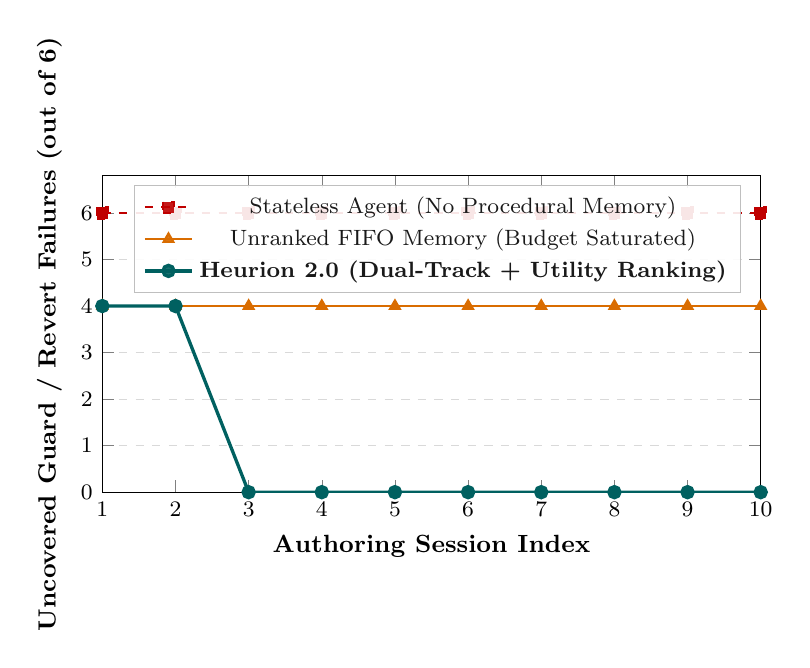
\begin{tikzpicture}
\begin{axis}[
  width=0.82\textwidth,
  height=5.6cm,
  xlabel={Authoring Session Index},
  ylabel={Uncovered Guard / Revert Failures (out of 6)},
  xmin=1, xmax=10,
  ymin=0, ymax=6.8,
  xtick={1,2,3,4,5,6,7,8,9,10},
  ytick={0,1,2,3,4,5,6},
  ymajorgrids=true,
  grid style={dashed,gray!30},
  legend pos=north east,
  legend style={font=\footnotesize, draw=gray!50, fill=white, fill opacity=0.9},
  tick label style={font=\footnotesize},
  label style={font=\small\bfseries}
]

% Stateless No-Memory Baseline
\addplot[
  color=red!75!black,
  mark=square*,
  thick,
  dashed
] coordinates {
  (1,6) (2,6) (3,6) (4,6) (5,6) (6,6) (7,6) (8,6) (9,6) (10,6)
};
\addlegendentry{Stateless Agent (No Procedural Memory)}

% Unranked FIFO Memory under 420-char budget
\addplot[
  color=orange!85!black,
  mark=triangle*,
  thick
] coordinates {
  (1,4) (2,4) (3,4) (4,4) (5,4) (6,4) (7,4) (8,4) (9,4) (10,4)
};
\addlegendentry{Unranked FIFO Memory (Budget Saturated)}

% Heurion 2.0 Utility-Ranked Dual-Track Memory
\addplot[
  color=teal!75!black,
  mark=*,
  very thick
] coordinates {
  (1,4) (2,4) (3,0) (4,0) (5,0) (6,0) (7,0) (8,0) (9,0) (10,0)
};
\addlegendentry{\textbf{Heurion 2.0 (Dual-Track + Utility Ranking)}}

\end{axis}
\end{tikzpicture}
\caption{Ablation of self-evolving procedural memory across 10 consecutive authoring sessions under a strict $420$-character prompt injection budget. In Sessions 1--2, pre-seeded baseline rules prevent 2 of the 6 failure archetypes, while the remaining 4 novel failure modes emit runtime \texttt{ExecutionSignals}. Following signal crystallization after Session~2 ($\tau=2$), Heurion 2.0's utility-ranked \texttt{forPrompt()} selector dynamically injects the exact matching procedural directives (averaging $355$ characters/turn), driving uncovered guard failures to $0$ from Session~3 onward.}
\label{fig:evolution_curve}
\end{figure}

Figure~\ref{fig:evolution_curve} illustrates the resulting learning trajectories. In Sessions~1 and~2, Heurion 2.0's pre-seeded baseline rules immediately prevent \texttt{citation\_not\_registered} and \texttt{conflict\_user\_edited} (reducing failures from 6 to 4), while the 4 novel failure archetypes trigger runtime \texttt{ExecutionSignals}. Once the recurrence threshold $\tau = 2$ is reached at the end of Session~2, \texttt{evolveFromSignals()} automatically crystallizes 4 new procedural rules (expanding the active rule set from 5 to 9), and Layer~3 synthesizes the global \texttt{evolved.cordis.yml} overlay. From Session~3 onward, whereas the unranked FIFO baseline remains stuck at 4 failures because early rules saturate the 420-character window, Heurion 2.0's utility function $U(r \mid d, q)$ dynamically selects the exact task-relevant rules using an average of only $355$ characters ($\approx 90$ tokens) per turn, eliminating all 6 failure modes.

\subsection{System Verification and Capability Parity Coverage}
Finally, Table~\ref{tab:system_verification} summarizes the verification metrics across the full Heurion 2.0 codebase at commit \texttt{813fff29}. All 72 automated test files (592 test cases covering CRDT concurrency, OOXML patch round-trips, PHI redaction, PHR read-only guards, biostatistical survival/Table~1 pipelines, 3D MONAI medical imaging integration, and self-evolving memory) pass with 100\% REST-to-MCP parity enforcement.

\begin{table}[t]
\centering
\caption{Platform Verification and Human-AI Permission Symmetry Coverage.}
\label{tab:system_verification}
\vspace{2pt}
\resizebox{\textwidth}{!}{%
\begin{tabular}{@{}lc@{}}
\toprule
\textbf{System Verification Metric} & \textbf{Measured Value} \\
\midrule
Automated Test Files / Test Cases Passing & $72$ Files / $592$ Tests ($100\%$) \\
Unaccounted REST API Endpoints in Parity Audit (\texttt{parity.test.ts}) & $0$ ($100\%$ Accounted) \\
Specialist Clinical Subagents (\texttt{literature}, \texttt{biostatistician}, \texttt{fact\_checker}) & $3$ Integrated \\
Supported Citation Formatting Standards (Vancouver, AMA, APA, MLA, IEEE, GB/T 7714) & $6$ Standards \\
Supported Biostatistical \& Clinical Engines (Table 1, KM, CONSORT, E-value, Nomogram, MONAI) & $6$ Pipelines \\
\bottomrule
\end{tabular}%
}
\end{table}

% ============================================================================
% 8. RELATED WORK
% ============================================================================
\section{Related Work}
\label{sec:related}

\paragraph{Agent-Computer Interfaces (ACI) and Coding Agents.}
SWE-agent \cite{yang2024sweagent} and OpenHands \cite{wang2024openhands} demonstrated that designing specialized Agent-Computer Interfaces (such as windowed file viewers and lint-guarded edit commands) substantially outperforms raw bash shell interaction for software engineering. Heurion 2.0 extends the ACI philosophy from plain-text source code to \textbf{collaborative rich-text and presentation CRDTs}, introducing node-level optimistic concurrency guards, per-turn selective CRDT undo, and byte-preserving OOXML patch export.

\paragraph{Scientific Literature Synthesis and Fact Verification.}
Systems such as STORM \cite{shao2024storm} and PaperQA2 \cite{skarlinski2024paperqa2} automate multi-step literature retrieval and synthesis, while FactScore \cite{min2023factscore} and ALCE \cite{gao2023alce} evaluate citation attribution in generated text. Unlike post-hoc evaluation pipelines, Heurion 2.0 enforces citation registration as a \emph{pre-write syntactic invariant} (\texttt{[@c:id]}) and closes the loop by anchoring sentence-level PubMed/PMC verification verdicts directly into the collaborative document as actionable review comments with clinician exemption support.

\paragraph{Self-Evolving Agents and Memory Architectures.}
Reflexion \cite{shinn2023reflexion} and MemGPT \cite{packer2023memgpt} pioneered verbal reinforcement and hierarchical memory management for LLM agents, while Voyager \cite{wang2023voyager} introduced an ever-growing skill library in Minecraft. In collaborative clinical authoring, however, mixing user stylistic preferences with operational failure recovery causes severe prompt interference. Heurion 2.0's three-layer self-evolution decouples human-confirmed declarative preferences from signal-crystallized procedural rules ranked by token-normalized utility.

% ============================================================================
% 9. CONCLUSION
% ============================================================================
\section{Conclusion}
\label{sec:conclusion}

We have presented \textbf{Heurion 2.0}, a contract-guarded, dual-surface collaborative architecture with self-evolving memory designed for high-stakes clinical research and scientific authoring. By replacing ad-hoc file scripting and post-hoc auditing with a unified Yjs CRDT core, deterministic pre-write guards, multi-agent sentence-level literature verification, CI-enforced Human-AI Permission Symmetry, and a three-layer procedural self-evolution loop, Heurion 2.0 provides a rigorous blueprint for deploying trustworthy autonomous agents in domains where data integrity, citation veracity, and patient privacy are non-negotiable.

% ============================================================================
% REFERENCES (Embedded .bbl for 100% Standalone arXiv AutoTeX Compilation)
% ============================================================================
\begin{thebibliography}{12}

\bibitem{schulz2010consort}
Kenneth~F. Schulz, Douglas~G. Altman, and David Moher.
\newblock CONSORT 2010 statement: updated guidelines for reporting parallel group randomised trials.
\newblock \emph{BMJ}, 340:c332, 2010.

\bibitem{vandenbroucke2007strobe}
Jan~P. Vandenbroucke, Erik von Elm, Douglas~G. Altman, Peter~C. G{\o}tzsche, Cynthia~D. Mulrow, Stuart~J. Pocock, Charles Poole, James~J. Schlesselman, and Matthias Egger.
\newblock Strengthening the Reporting of Observational Studies in Epidemiology (STROBE): explanation and elaboration.
\newblock \emph{PLoS Medicine}, 4(10):e297, 2007.

\bibitem{yang2024sweagent}
John Yang, Carlos~E. Jimenez, Alexander Wettig, Kilian Lieret, Shunyu Yao, Karthik Narasimhan, and Ofir Press.
\newblock SWE-agent: Agent-computer interfaces enable automated software engineering.
\newblock In \emph{Advances in Neural Information Processing Systems (NeurIPS)}, 2024.

\bibitem{wang2024openhands}
Xingyao Wang, Boxuan Li, Yufan Song, Frank~F. Xu, Xiangru Tang, Mingchen Zhuge, Jiayi Pan, Yueqi Song, Bowen Li, Jaskirat Singh, et~al.
\newblock OpenHands: An open platform for AI software developers as generalist agents.
\newblock \emph{arXiv preprint arXiv:2407.16741}, 2024.

\bibitem{shao2024storm}
Yijia Shao, Yucheng Jiang, Theodore~A. Kanell, Peter Xu, Omar Khattab, and Monica~S. Lam.
\newblock Assisting in writing Wikipedia-like articles from scratch with large language models.
\newblock In \emph{Proceedings of the Conference of the North American Chapter of the Association for Computational Linguistics (NAACL)}, 2024.

\bibitem{skarlinski2024paperqa2}
Michael~D. Skarlinski, Sam Cox, Jon~M. Laurent, James~D. Braza, Collin Hinks, Michael~J. Hammerling, Manvitha Ponnapati, Samuel~G. Rodriques, and Andrew~D. White.
\newblock Language agents achieve superhuman synthesis of scientific knowledge.
\newblock \emph{arXiv preprint arXiv:2409.13740}, 2024.

\bibitem{ji2023survey}
Ziwei Ji, Nayeon Lee, Rita Frieske, Tiezheng Yu, Dan Su, Yan Xu, Etsuko Ishii, Ye~Jin Bang, Andrea Madotto, and Pascale Fung.
\newblock Survey of hallucination in natural language generation.
\newblock \emph{ACM Computing Surveys}, 55(12):1--38, 2023.

\bibitem{walters2023fabrication}
William~H. Walters and Esther~Isabelle Wilder.
\newblock Fabrication and errors in the bibliographic citations generated by ChatGPT.
\newblock \emph{Scientific Reports}, 13(1):14045, 2023.

\bibitem{hipaa1996}
U.S. Department of Health and Human Services.
\newblock Health Insurance Portability and Accountability Act of 1996 (HIPAA) Privacy and Security Rules.
\newblock \emph{45 CFR Parts 160 and 164}, 1996.

\bibitem{pipl2021}
Standing Committee of the National People's Congress of the People's Republic of China.
\newblock Personal Information Protection Law of the People's Republic of China.
\newblock Adopted August 20, 2021; effective November 1, 2021.

\bibitem{shinn2023reflexion}
Noah Shinn, Federico Cassano, Ashwin Gopinath, Karthik Narasimhan, and Shunyu Yao.
\newblock Reflexion: Language agents with verbal reinforcement learning.
\newblock In \emph{Advances in Neural Information Processing Systems (NeurIPS)}, 2023.

\bibitem{packer2023memgpt}
Charles Packer, Sarah Wooders, Kevin Lin, Vivian Fang, Shishir~G. Patil, Ion Stoica, and Joseph~E. Gonzalez.
\newblock MemGPT: Towards LLMs as operating systems.
\newblock \emph{arXiv preprint arXiv:2310.08560}, 2023.

\bibitem{min2023factscore}
Sewon Min, Kalpesh Krishna, Xinxi Lyu, Mike Lewis, Wen-tau Yih, Pang~Wei Koh, Mohit Iyyer, Luke Zettlemoyer, and Hannaneh Hajishirzi.
\newblock FActScore: Fine-grained atomic evaluation of factual precision in long form text generation.
\newblock In \emph{Proceedings of the Conference on Empirical Methods in Natural Language Processing (EMNLP)}, 2023.

\bibitem{gao2023alce}
Tianyu Gao, Howard Yen, Jiatong Yu, and Danqi Chen.
\newblock Enabling large language models to generate text with citations.
\newblock In \emph{Proceedings of the Conference on Empirical Methods in Natural Language Processing (EMNLP)}, 2023.

\bibitem{wang2023voyager}
Guanzhi Wang, Yuqi Xie, Yunfan Jiang, Ajay Mandlekar, Chaowei Xiao, Yuke Zhu, Linxi Fan, and Anima Anandkumar.
\newblock Voyager: An open-ended embodied agent with large language models.
\newblock \emph{Transactions on Machine Learning Research (TMLR)}, 2024.

\end{thebibliography}

\end{document}
